%!TEX root=./main.tex

\section{Introduction}
A laparoscopic surgeon consults pre-operative images such as MR or CT to localize hidden  structures such as tumors and major vessels. However, it can be difficult, even for experienced surgeons, to accurately predict their positions during surgery. 
One of the main goals of CAI is to ease this task by enriching laparoscopic images with data from pre-operative MR or CT using AR~\cite{1732,8714}. 
%For example, systems have been proposed to visualize sub-surface structures~\cite{Simpfendrfer2011}, to enlarge the surgical field of view~\cite{Totz2011}, and to overlay information from other imaging modalities~\cite{Nakamoto2008}.
The key technical challenge is non-rigid registration of soft-body organs. Once achieved, the position of the hidden structures can be augmented onto the laparoscopic video. A major open challenge is achieving registration accurately, reliably and in real-time. 

We present the first complete AR pipeline for the uterus using a segmented pre-operative 3D model and monocular laparoscopic images, with novel technical contributions at various stages. This facilitates important clinical applications, including AR-assisted resection of lesions such as uterine fibroids. We specifically target monocular laparoscopes because their use is far more widespread than stereo laparoscopes in standard (non-robotic) laparoscopic procedures. This is because of several factors including
cost, setup time, image resolution, port size
and display comfort. However, the technical challenges are \SG{much} greater with monocular laparoscopes. 

The main phases of our AR pipeline are illustrated in Fig.~\ref{fig:processOverview} and explained in detail in \S3. Pre-operatively, the uterus is segmented from an MR image and its deformation properties are modelled. Intra-operatively, first, automatic \emph{camera calibration} is performed to determine the laparoscope's intrinsics such as its focal length, by withdrawing the scope from the patient and viewing a hand-held calibration planar \SG{target} (OpenCV). Next is \emph{scene exploration}, where the laparoscope is re-inserted and the uterus surface is viewed by movement of the laparoscope and uterus. Next is \emph{scene reconstruction}, where the uterus surface is reconstructed in 3D using dense multi-view-stereo (MVS). Next is \emph{initial registration}, where a 3D registration is performed to align the uterus model to the interventional reconstruction. Next is \emph{feature mapping}, where texture, in the form of keypoints such as SIFT \cite{Lowe:2004:DIF:993451.996342} or SURF \cite{SURF}, is associated to the model's surface. Finally, is \emph{tracking and AR}, where the model is tracked in real-time using robust keypoint matching with the laparoscope live video, and the registered model is visualized to the surgeon via AR. Our main contributions concentrate on the challenging problems of initial registration, feature mapping and tracking. 

\begin{figure}[t]
	\centering
	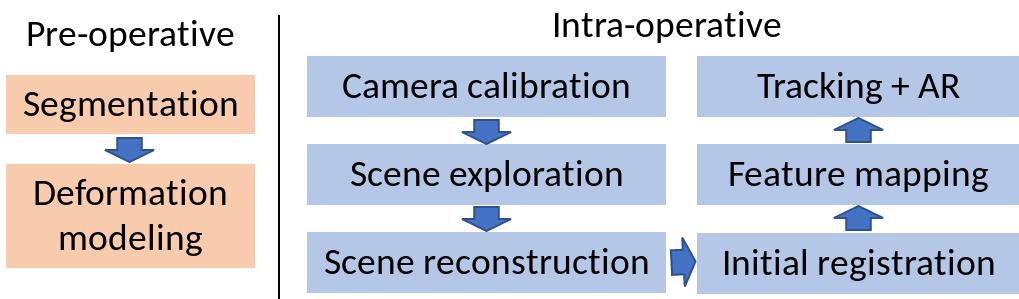
\includegraphics[width=0.8\columnwidth]{./figs/overview.png}
	\caption{Main phases of our AR pipeline}
	\label{fig:processOverview}
\end{figure}



%Most previous approaches for other organs have been developed for robotic surgery equipped with stereo laparoscopes~\cite{Schwab2017} and less commonly for monocular laparoscopes~\cite{nosrati2014simultaneous,haouchine:hal-01186011,affineTracking}. The challenges with the latter are far greater due to the lack of depth information. 
%However, there is a strong clinical need for the latter because monocular laparoscopes are the most common type in today's laparosurgery, 

%The proposed pipeline breaks down the registration problem in two stages.
%The first stage, the \emph{initial registration}, is non-live and it relies on Structure-from-Motion (SfM)~\cite{Hartley2004} and Multi-View Stereo (MVS)~\cite{Furukawa2015} to obtain a 3D dense model of the uterus from a laparoscopic image sequence. 
%We then register the dense model to the pre-operative model using a semi-automatic, non-rigid registration method that determines the change of state of the organ between its pre-operative state and the intra-operative initial state. 
%The second stage is \emph{real-time tracking}, performed in real-time, that registers new laparoscopic video frames to the model. The camera position is estimated \wrt the previously registered dense model, thus enabling image augmentation.
%Unlike most other approaches, we solve this by tracking-by-detection \emph{tracking-by-detection}, which does not rely on correct registration in previous frames. The proposed pipeline is robust to major challenges including occlusions and, contrary to other approaches such as the SLAM-based ones, it can handle a mobile organ.

%The paper is organized as follows: \sect{sec:sota} reviews the existing works in the literature, detailing why they are insufficient for solving registration with a mobile organ such as the uterus and our novel technical contributions. \sect{sec:ARGuidanceSystem} presents an overview of the proposed system, \sect{sec:initialRegistration} and \sect{sec:updateRegistration} detail the two main technical contributions of the paper, the registration and the real-time tracking algorithms respectively. 
%\sect{sec:experiments} presents the experiments that validate the proposed work and \sect{sec:conclusion} concludes the paper with future perspectives and improvements.